\documentclass[]{IEEEphot}
\jvol{1}
\jnum{1}
\jmonth{Marth}
\pubyear{2012}
\usepackage{graphicx}
\usepackage{fontspec}
\XeTeXlinebreaklocale "zh" %针对中文进行断行
\setmainfont{WenQuanYi Zen Hei} %设置默认的字体
\linespread{1.2}

\begin{document}
\title{数字图像处理实验一\\实验报告}
\author{040920112 戴一冕}
\maketitle
\markboth{数字图像处理}{实验一实验报告}
\begin{abstract}
  对给定实验图片进行图像反转、幂次变换和分段线性变换这些基本的灰度变换
\end{abstract}
\begin{IEEEkeywords}
	灰度变换,图像反转,幂次变换,分段线性变换,灰度切片
\end{IEEEkeywords}
\section{实验目的}
通过上机实验的手段巩固课堂上所学的关于图像反转、幂次变换和分段线性变换有关的知识,感受不同的灰度变换方法对最终图像效果的影响。
\section{实验内容}
\subsection{方法技术介绍}
灰度变换函数是图像增强技术中最简单的一类,处理前后的像素值分别用$r$和$s$定义,于是我们可以如下表达式来表示原像素值$r$映射到值$s$的变换:
\begin{equation}
	s = T(r)
	\label{eql}
\end{equation}
\subsubsection{图像反转}
灰度级范围为[0,L-1]的图像反转表达式为: 
\begin{equation}
	s = L-1-r
	\label{eql}
\end{equation}
采用上式可以产生图像反转的对等图像,这种处理尤其适合用于增强嵌入于图像暗色区域的白色或灰色细节,特别是当黑色面积占主导地位时。
\subsubsection{幂次变换}
幂次变换的基本形式为:
\begin{equation}
	s = cr^{\gamma}
	\label{eql}
\end{equation}
其中$c$和$\gamma$为正常数。从下图可以看出,当${\gamma}<{1}$,幂次变换能够将窄带暗值映射成宽带输出值,${\gamma}>{1}$,则正好相反。应注意的是,当$c={\gamma}=1$时,幂次变换将简化为正比运算。
\begin{figure}[h]
\centering
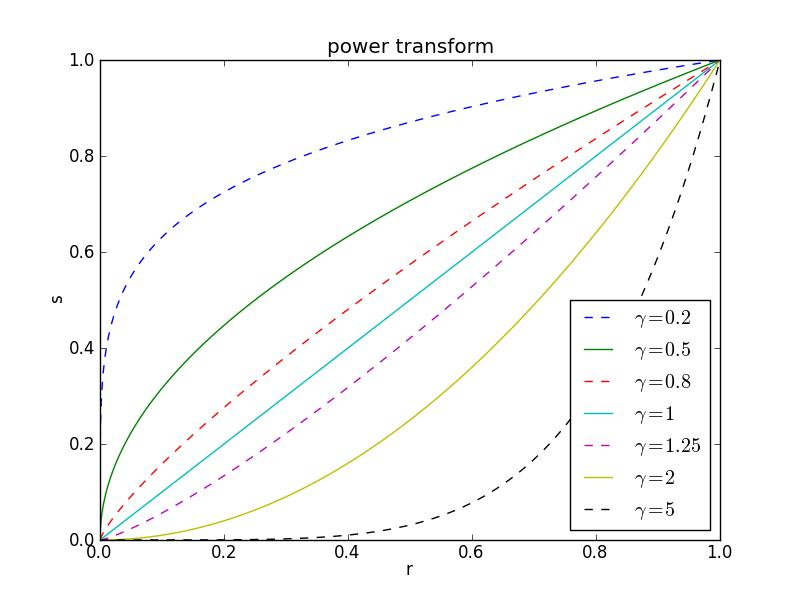
\includegraphics[width=21pc]{power_trans.eps}\\
\label{fig_envl}
\end{figure}
\subsubsection{分段线性变换}
与前面两个函数相比,分段线性变换的主要优势在于形式可以任意合成,其中分段线性变换还可以细分为对比拉伸、灰度切割、位图切割等方法。
\paragraph{对比拉伸}
对比拉伸的思想是提高低对比度图像处理是灰度级的动态范围。低对比度的成因有照明不足、成像传感器动态范围太小,甚至在图像获取过程中透镜光圈设置错误引起。
\paragraph{灰度切割}
在图像处理中提高特定灰度范围的亮度通常是很有必要的,这样的灰度切割可以让感兴趣的图像内容更加明显。
\subsection{实验步骤}
\subsubsection{步骤1}
用PIL中的Image.open方法获取实验用图:rice.png,使用convert('L')方法将其变为灰度图像。再通过numpy的asarray方法将其转化为numpy数组,以便后续的操作。
\subsubsection{步骤2}
用如下的灰度变换函数对rice.png图像进行处理。
\begin{equation}
	s = \left\{
		\begin{array}{lr}
			0.3r, & r < 0.35 \\
			0.105 + 2.6333(r-0.35), & 0.35\leq r \leq 0.65\\
					  1 + 0.3(r-1), & r > 0.65.
		\end{array}
		\right.
		\label{eql}
\end{equation}
\subsubsection{步骤3}
用如下灰度变换函数对rice.png进行处理。
\begin{equation}
	s = \left\{
		\begin{array}{lr}
			15.9744r^5, & r \leq 0.5 \\
	(r-0.5)^{0.2}+0.12, & r > 0.5 
		\end{array}\right.
		\label{eql}
	\end{equation}
\subsubsection{步骤4}
分别用$s=r^{0.6}$ $s=r^{0.4}$ $s=r^{0.3}$ 对kids.tif图像进行处理。
\subsubsection{步骤5}
对circuit.jpg图像实施反变换。
\subsubsection{步骤6}
对rice.jpg图像实施灰度切片。具体要求为:当$0.2\leq r\leq 0.4$时,将$r$置为0.6,当$r$位于其他区间时,保持其灰度值不变。
\subsubsection{步骤7}
利用灰度变换对Picture.jpg做增强处理,突出图中人物,改善整个图像过于灰暗的背景。给出图像处理前后的直方图,写出所采用的拉伸表达式。
\section{实验结果与分析}
\subsection{实验环境介绍}
本实验采用Python 2.7.2及其Numpy、Scipy、PIL、matplotlib,以及笔者自己编写的PyDIP模块,同时又用Matlab再实验了一次以用来对照。
\subsection{分析结果}
\subsubsection{步骤1}
matplotlib中的imshow函数,默认是将灰度图像用伪彩色显示,故而还需导入matplotlib.cm模块,显式的将imshow的cmap参数设置为cm.gray。对于Numpy,Scipy,PIL,matplotlib等模块可以在其官网上很方便的下载,而对于我自己写的PyDIP模块则可以从github的PyDSP项目下下载到。
\subsubsection{步骤2}
\begin{figure}[h]
\centering
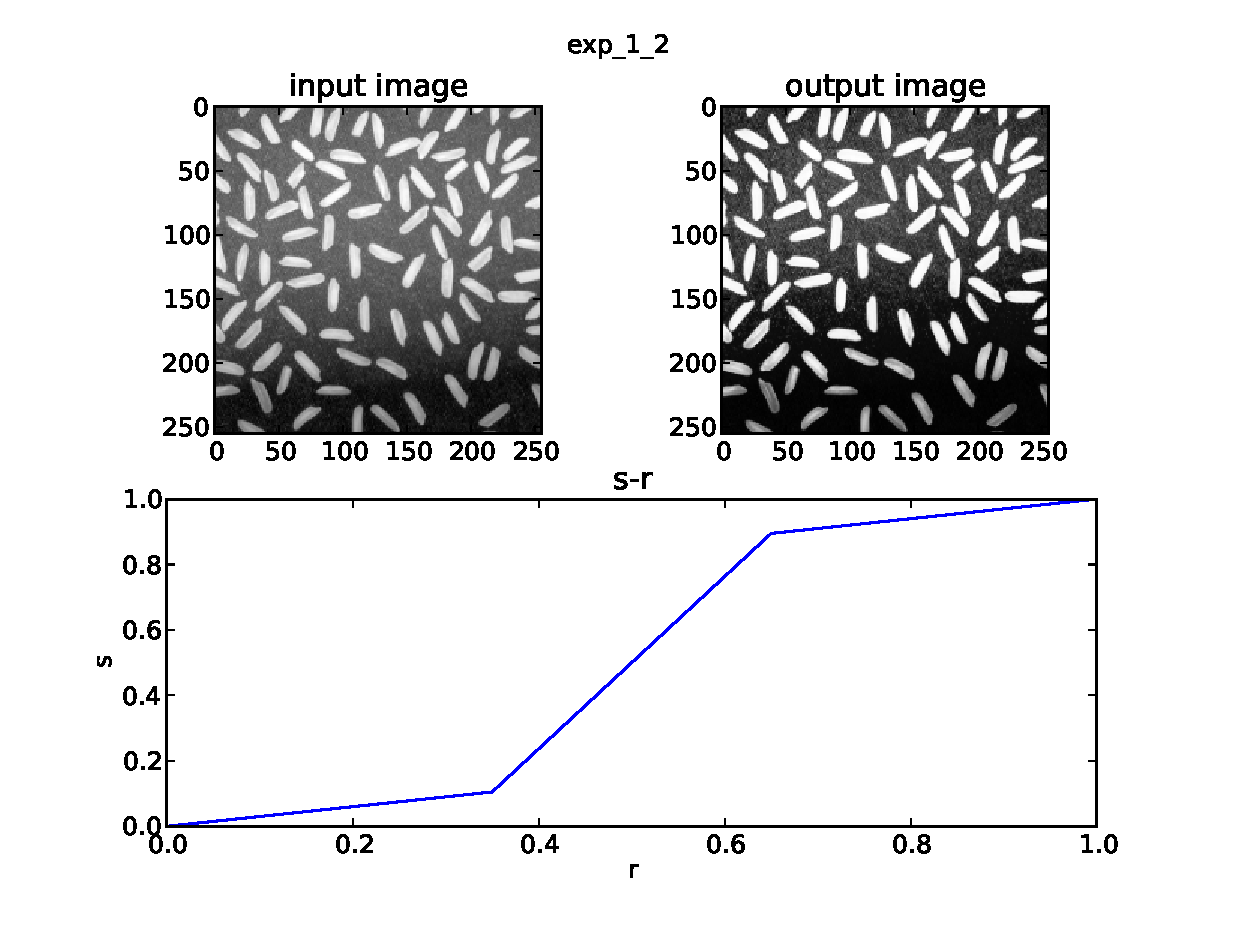
\includegraphics[width=21pc]{exp_1_2.eps}\\
\label{fig_env2}
\end{figure}
该步骤在图像灰度变换中属于分段线性变换,在$r<0.35$和$r>0.65$的范围内,斜率$\frac{ds}{dr}$均小于$1$,这样操作的效果是令图像灰度分布有两极化的趋势,从而增强图像的对比度。
\subsubsection{步骤3}
\begin{figure}[h]
\centering
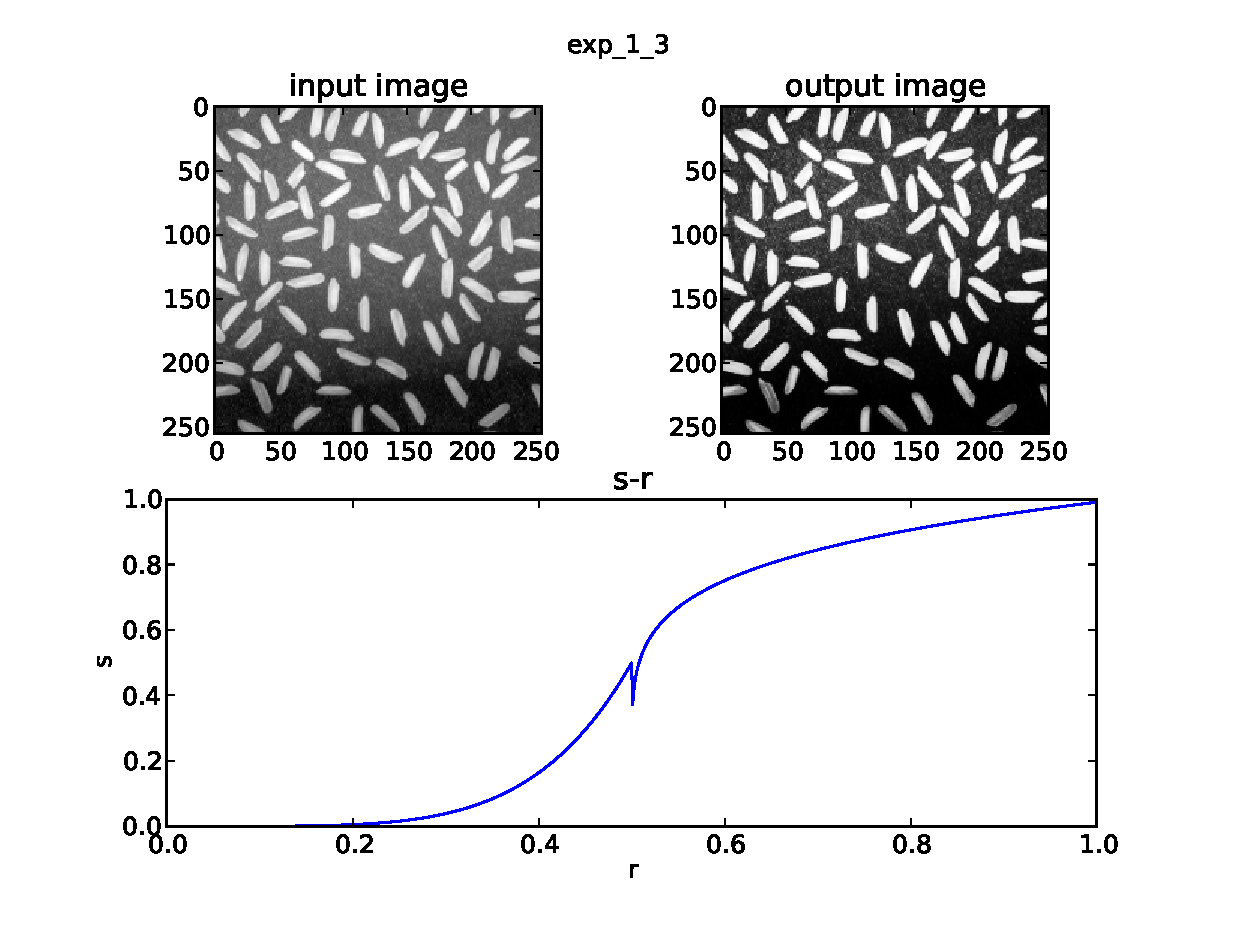
\includegraphics[width=21pc]{exp_1_3.eps}\\
\label{fig_env2}
\end{figure}
该步骤的灰度变换函数很难简单的说是属于那种类型,应该是幂次变换和分段线性的混合体。虽然类型怪异,但是其目的和效果还是和步骤一相同的,均是让图像灰度分布有两极化趋势,从而增强图像的对比度。
\subsubsection{步骤4}
\begin{figure}[h]
\centering
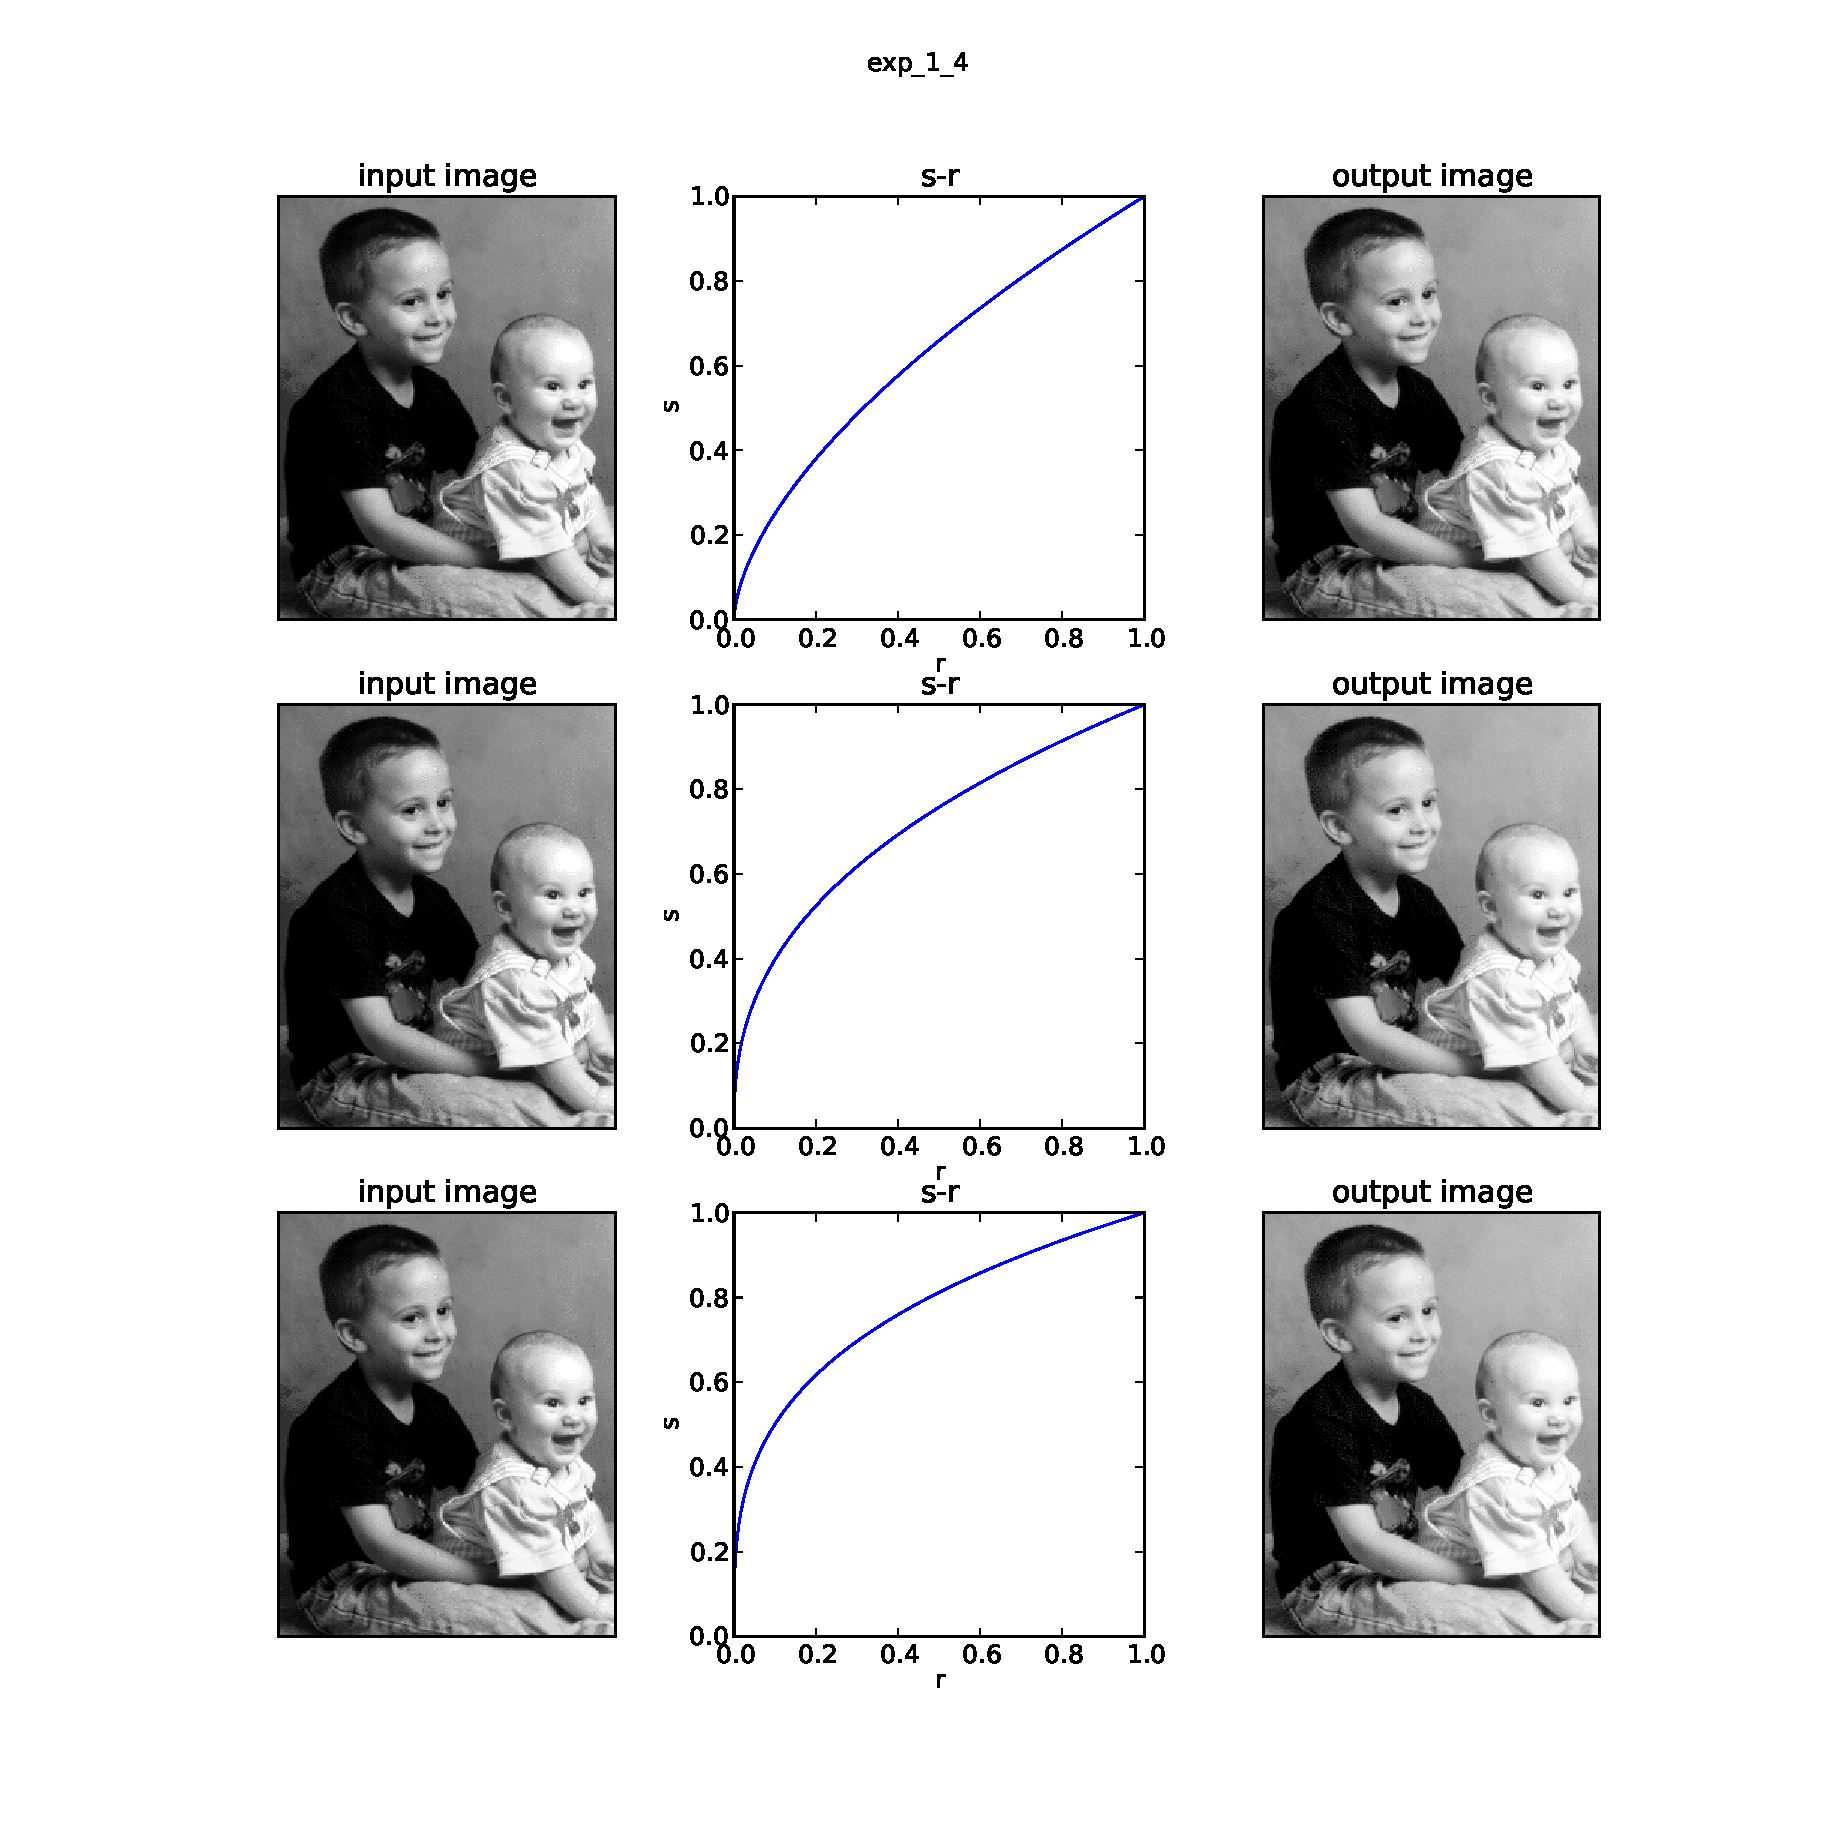
\includegraphics[width=21pc]{exp_1_4.eps}\\
\label{fig_env2}
\end{figure}
该步骤是典型的幂次变换,从上文中容易知道,$\gamma$越小,变换后的图像整体灰度值偏高,实验结果中输出图片整体都比原图要亮,且越是下面的图片也越是亮也正好反应了这一点。
\subsubsection{步骤5}
\begin{figure}[h]
\centering
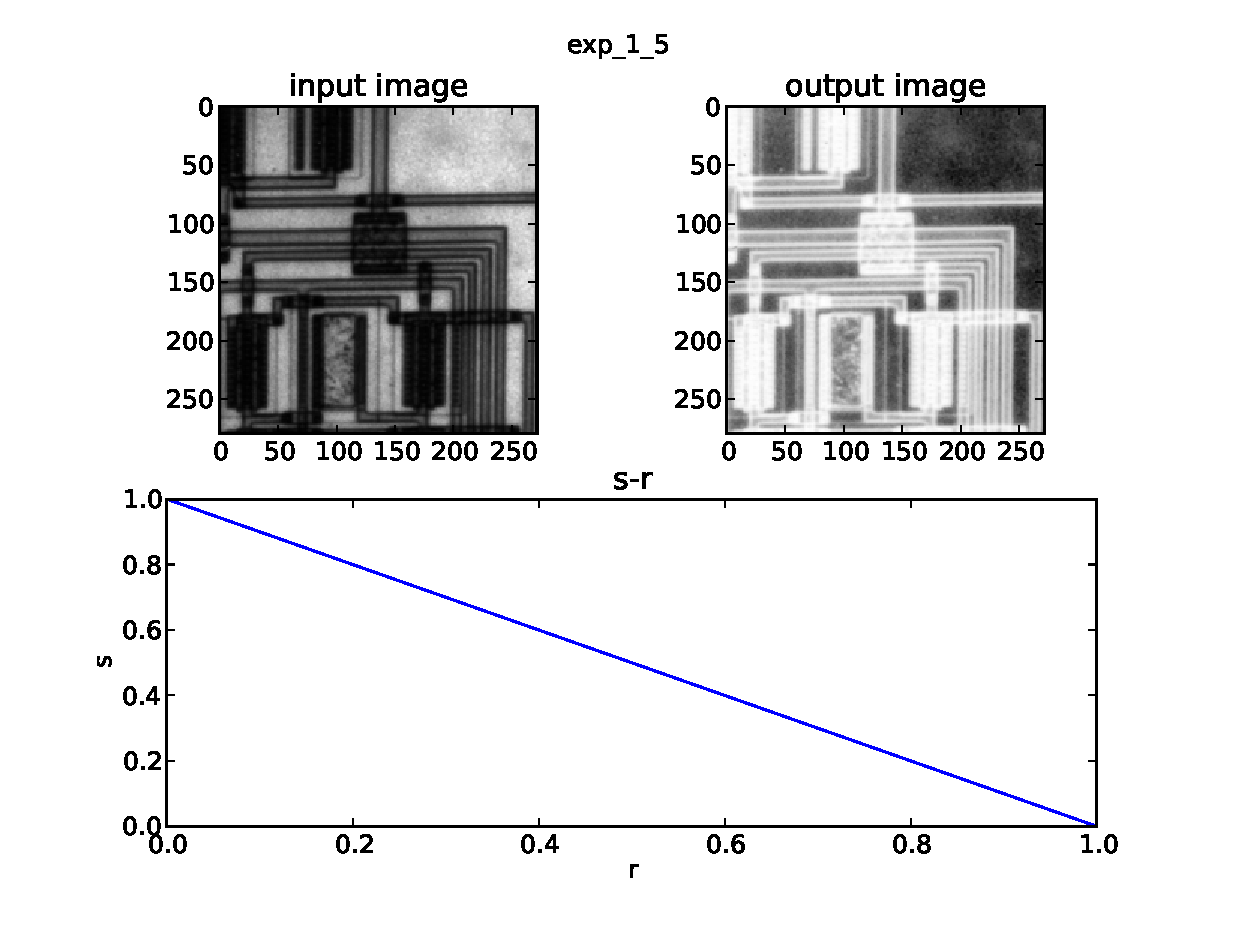
\includegraphics[width=21pc]{exp_1_5.eps}\\
\label{fig_env2}
\end{figure}
该步骤属于灰度变换中的图像反转,对于读入的uint8类型的二维数组来说,就是每个数组的每个元素进行:
$$ s=L-1-r=256-1-6=255-r$$
对于浮点类型来说,就是:
$$s=1-r$$
图像反转通常应用的场景是,目标区域为较暗难以分辨的区域,而周边的区域则较为明亮,这样不容易观察。进行图像反转后则正好可以突出目标区域。
\subsubsection{步骤6}
\begin{figure}[h]
\centering
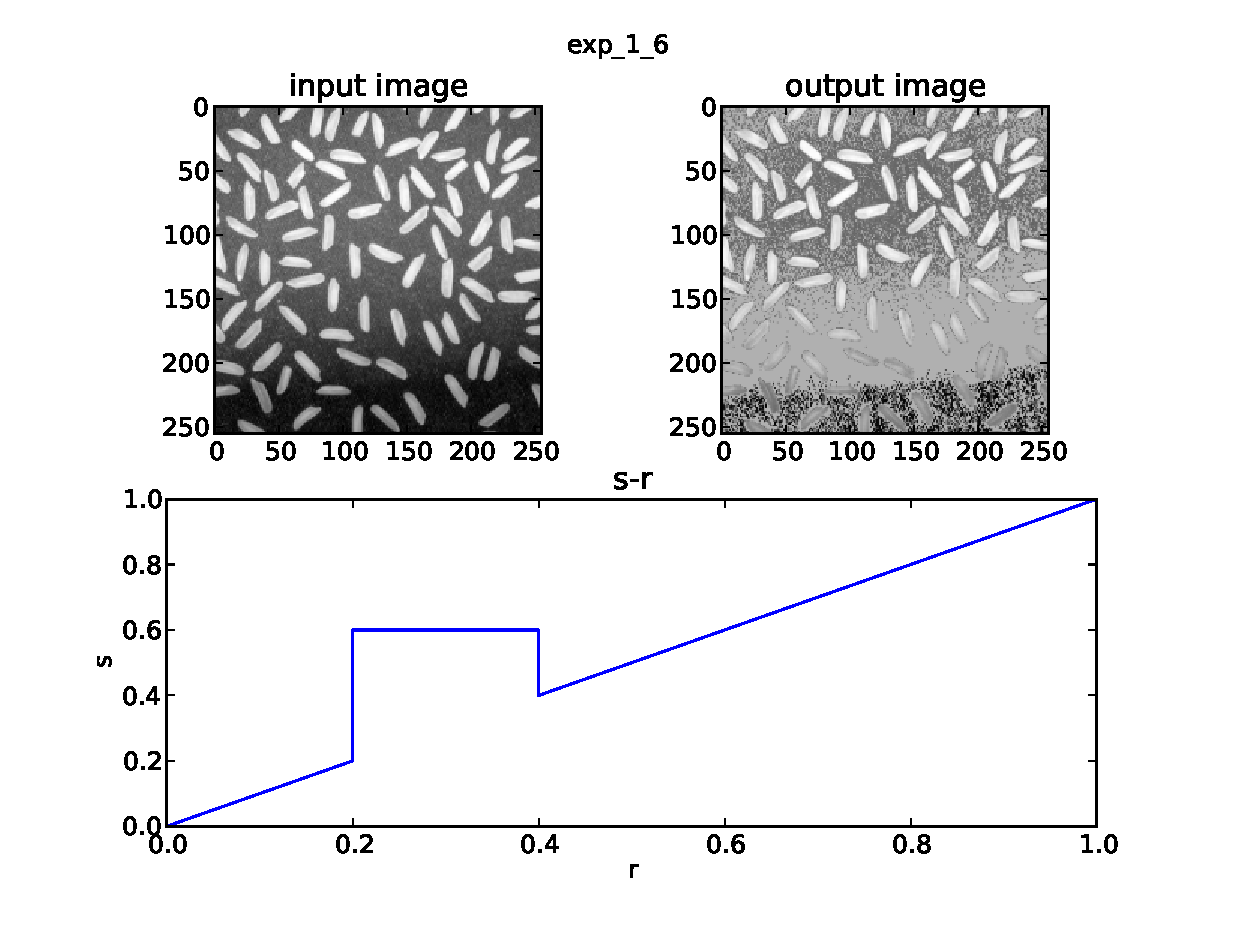
\includegraphics[width=21pc]{exp_1_6.eps}\\
\label{fig_env2}
\end{figure}
该步骤属于灰度切割,目的是增强$r\in[0.2,0.4]$这段关心范围内的灰度值,从而使该区间更为明显。
\subsubsection{步骤7}
由于原图像的整体灰度值偏小,主要集中在[0,50]中间,背景和人物相差不明显。虽然没有要求采用直方图均衡而是分段线性拉伸来处理,但我想直方图均衡的目的是让图像的灰度值分布均匀,从而使信息熵最大,相应的图像对比度也会增强,背景和人物也就易于区分。
那么对于本图像的分段线性变换,用人去判断究竟是哪种分段线性函数更能让背景和人物区别开来是很主观的,观看变换前后两图像的直方图分布,是较为客观的。于是我从让直方图分布均衡的角度出发,尝试不同的分段线性变换函数,择取如下函数作为最终的结果。
\begin{equation}
	s=\left\{
		\begin{array}{lr}
			4r,& 0\leq r<25\\
  2(r-25)+100, & 25\leq r<50\\
			\frac{105}{205}(r-50)+150, & 50\leq r\leq 255
		\end{array}
		\right.
		\label{eql}
	\end{equation}
\begin{figure}
\centering
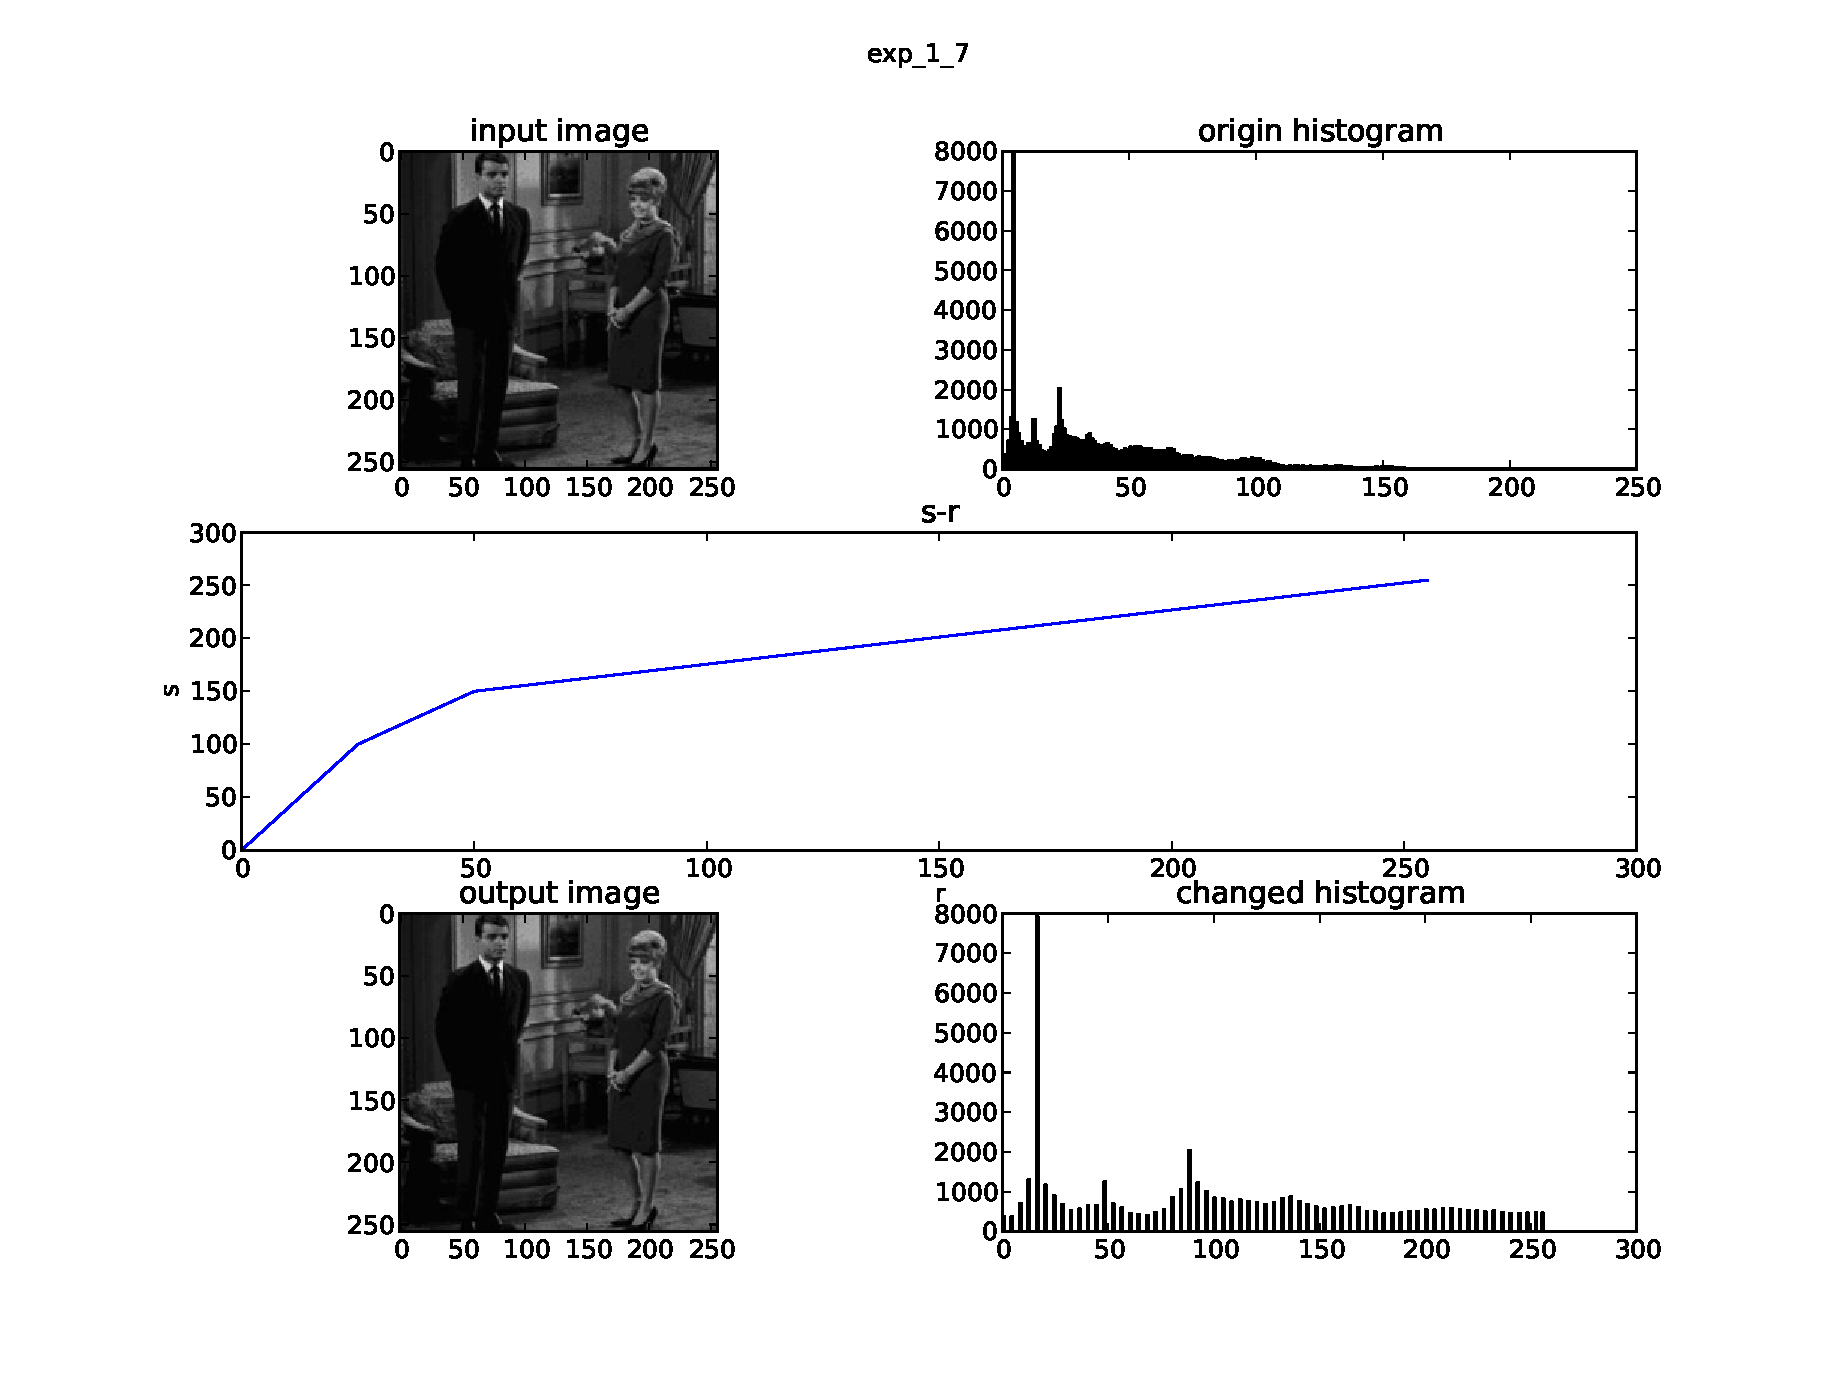
\includegraphics[width=40pc]{exp_1_7.eps}\\
\label{fig_env2}
\end{figure}
在实验过程中,发现PIL并没有用于绘制灰度直方图的方法,但利用numpy的histogram函数可以用来统计灰度情况,在利用matplotlib.pylab中的bar绘图函数即可。需要指出的是,在用histogram统计前,需先将表示图像的二维数组折叠成一维,如果图像本来就是numpy数组,即可直接调用flatten函数,新的pyopencv 2.x中也将默认读入图像从mat改为了ndarray。
\section{心得体会}
这次实验,让我更加深入的理解了图像反转、幂次变换、图像拉伸、分段线性变换这些基本的空域增强方法,是对课堂教学的一次很好的补充。不由感叹,如果在大二刚开始上专业课的时候对于信号与系统、电路分析这些专业课如果也有相应的需要自己编程的实验的话,我们对那些基础知识的掌握也许会更好。
还有就是选择一门合适编程语言真的是很重要。我先用matlab语言写完了本实验,但是对实验内容的体会并不深,采用了Python后,虽然Python也有相应的图像处理类库,但本次实验我没有采用pyopencv,而是采用了PIL,跟matlab的image processing box比起来简直就是小巫见大巫。函数库的不完全也是有好处的,需要自己动手写图像处理相关的函数,这更加加深了我对课堂知识的理解。
\section{实验程序}
实验的程序可以在随文的文件夹内找到。
\end{document}

